\section{Background}
In recent years, with the wide application of new technologies such as mobile smart 
devices and cloud computing. People are communicating more and more through the Internet. 
The e-commerce and online transactions are becoming more and more popular. Our human 
beings are moving towards into a digital society\cite{b2}. In order to guarantee the confidentiality, 
integrity, availability and authenticity of data in various network activities in digital 
society, various modern cryptographic techniques have been widely adopted, especially 
public key cryptography, which has become the core of security to ensure the Internet and 
the whole digital society\cite{b1}. Compared with traditional symmetric cryptography, public key 
cryptography not only realizes data encryption and message authentication, but also user 
authentication, digital signature, secure computing, key exchange, verifiable secret 
sharing and other functions, which lays a solid security foundation for ensuring the 
development of new Internet business\cite{b4}.
\\
Many people mistakenly believe that decentralization, the reason why it sits on a 
large number of supporters, is because it can resist government censorship, help 
users to use financial services freely and comfortably. In addition, it can realize the vision of 
universal financial services\cite{b3}.
\\
However, the advantages of decentralization don't stop there -- the most important 
aspect is that it provides greater protection for user privacy\cite{b16}.

\begin{figure}[H] %H为当前位置,!htb为忽略美学标准,htbp为浮动图形
\centering %图片居中
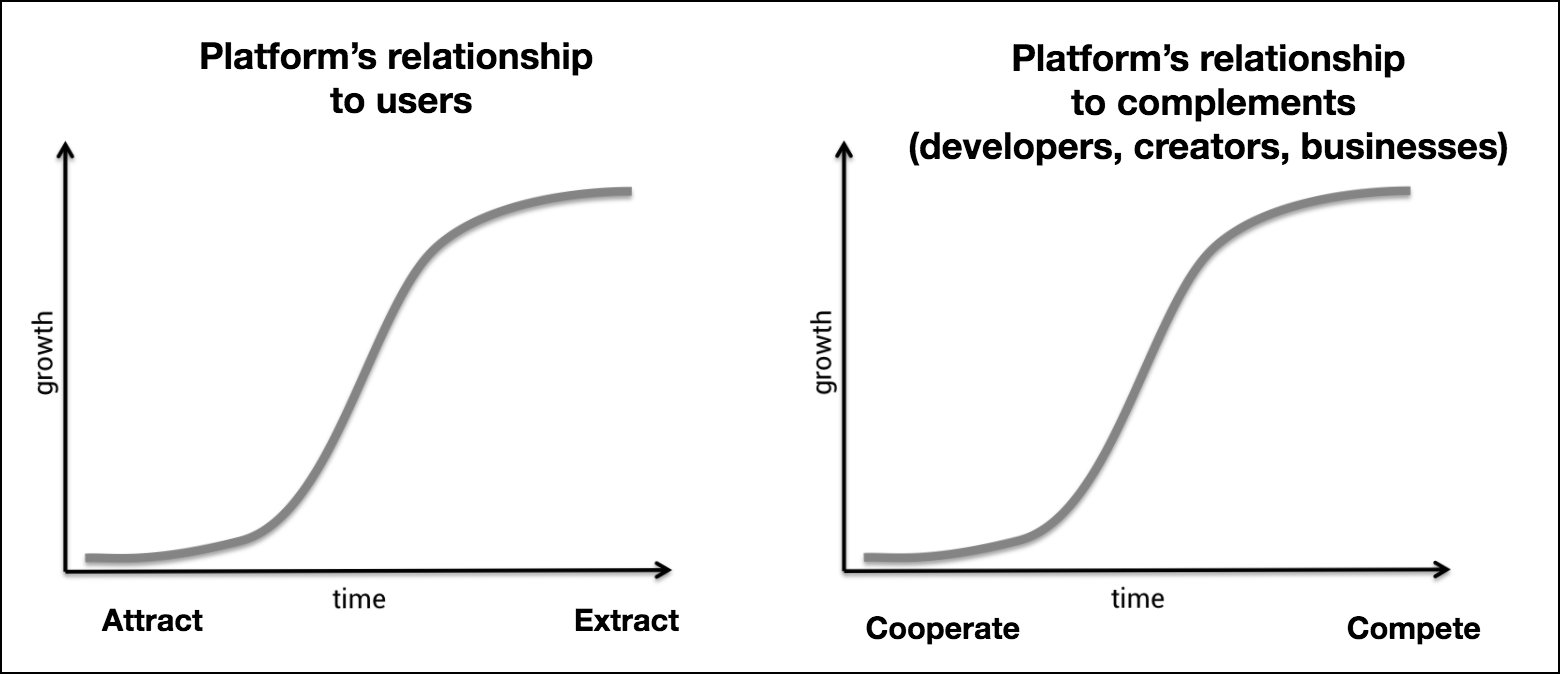
\includegraphics[width=0.5\textwidth]{figures/media.png} %插入图片,[]中设置图片大小,{}中是图片文件名
\caption{lifecycle of a centralized platform} %最终文档中希望显示的图片标题
\label{Fig.1: lifecycle of a centralized platform} %用于文内引用的标签
\end{figure}

\\
The diagram above illustrates the lifecycle of a centralized platform\cite{b35}. When most 
centralized platforms start out, they do everything in their power to engage users 
and third parties such as developers, creators, and businesses in order to increase 
the value and penetration of their services. As the centralized platform develops in 
an S-curve, the power of the platform over the participants rises, gradually weakening 
the users' control over their personal information\cite{b34}.
\\
Once it reaches the top of the S-curve, the relationship between the centralized 
platform and its users shifts from Positive-sum to Zero-sum\cite{b35, b17, b18}. In order to continue 
to expand, centralized platforms often sell user data to third parties other than 
users to make further profits. The most widely known examples are iOS and Android\cite{b34}, 
where developers must pay up to 30\% of their profits if they want to reach the 
platform's audience and sell apps in the Apple Store or Google Play\cite{b33}.
Due to a new bill in Europe that restricts the major application platforms, such as Apple Store.
However, they can still receive over 15\% of the benefits\cite{b39}.
\\
This not only affects the confidence of developers and creators in centralized platforms, 
but also sacrifices the privacy of users, leading to more security breaches and 
information security incidents, which are likely to become more frequent and serious 
as centralized platforms evolve\cite{b34}.
\\
For example, in April 2021, as many as 533 million pieces of Facebook data, 
such as phone numbers, names, and email addresses, were compromised by hackers, making 
it the largest data breach in recent years\cite{b32}.